%% LyX 2.1.4 created this file.  For more info, see http://www.lyx.org/.
%% Do not edit unless you really know what you are doing.
\documentclass[american]{article}
\usepackage[T1]{fontenc}
\usepackage{algorithm2e}
\usepackage{amsmath}
\usepackage{graphicx}

\makeatletter
%%%%%%%%%%%%%%%%%%%%%%%%%%%%%% User specified LaTeX commands.
\usepackage{amsmath}
\DeclareMathOperator*{\argmax}{arg\,max}
\DeclareMathOperator*{\argmin}{arg\,min}

\makeatother

\usepackage{babel}
\begin{document}

\title{Relative Edge Optimization Jacobian Derivation}


\author{James Jackson, David Wheeler}

\maketitle
As a reference, the cost function for relative edge optimization is

\[
\begin{aligned}\begin{aligned}F(\mathbf{\hat{z}}, & \mathbf{\bar{z}})\end{aligned}
 & =\sum_{\{i,j\}\in\mathcal{O}}\end{aligned}
(\mathbf{\hat{z}}_{ij}-\bar{\mathbf{z}}_{ij})^{\top}\Omega_{i,j}(\mathbf{\hat{z}}_{ij}-\bar{\mathbf{z}}_{ij})+\sum_{\{a,z\}\in\mathcal{L}}(\mathbf{\hat{z}}_{a-z}-\bar{\mathbf{z}}_{az})^{\top}\Omega_{az}(\mathbf{\hat{z}}_{a-z}-\bar{\mathbf{z}}_{az})
\]



\section{Specific Example}

Let's consider a pose graph with the configuration shown in Figure
1.

\begin{figure}[h]
\caption{\protect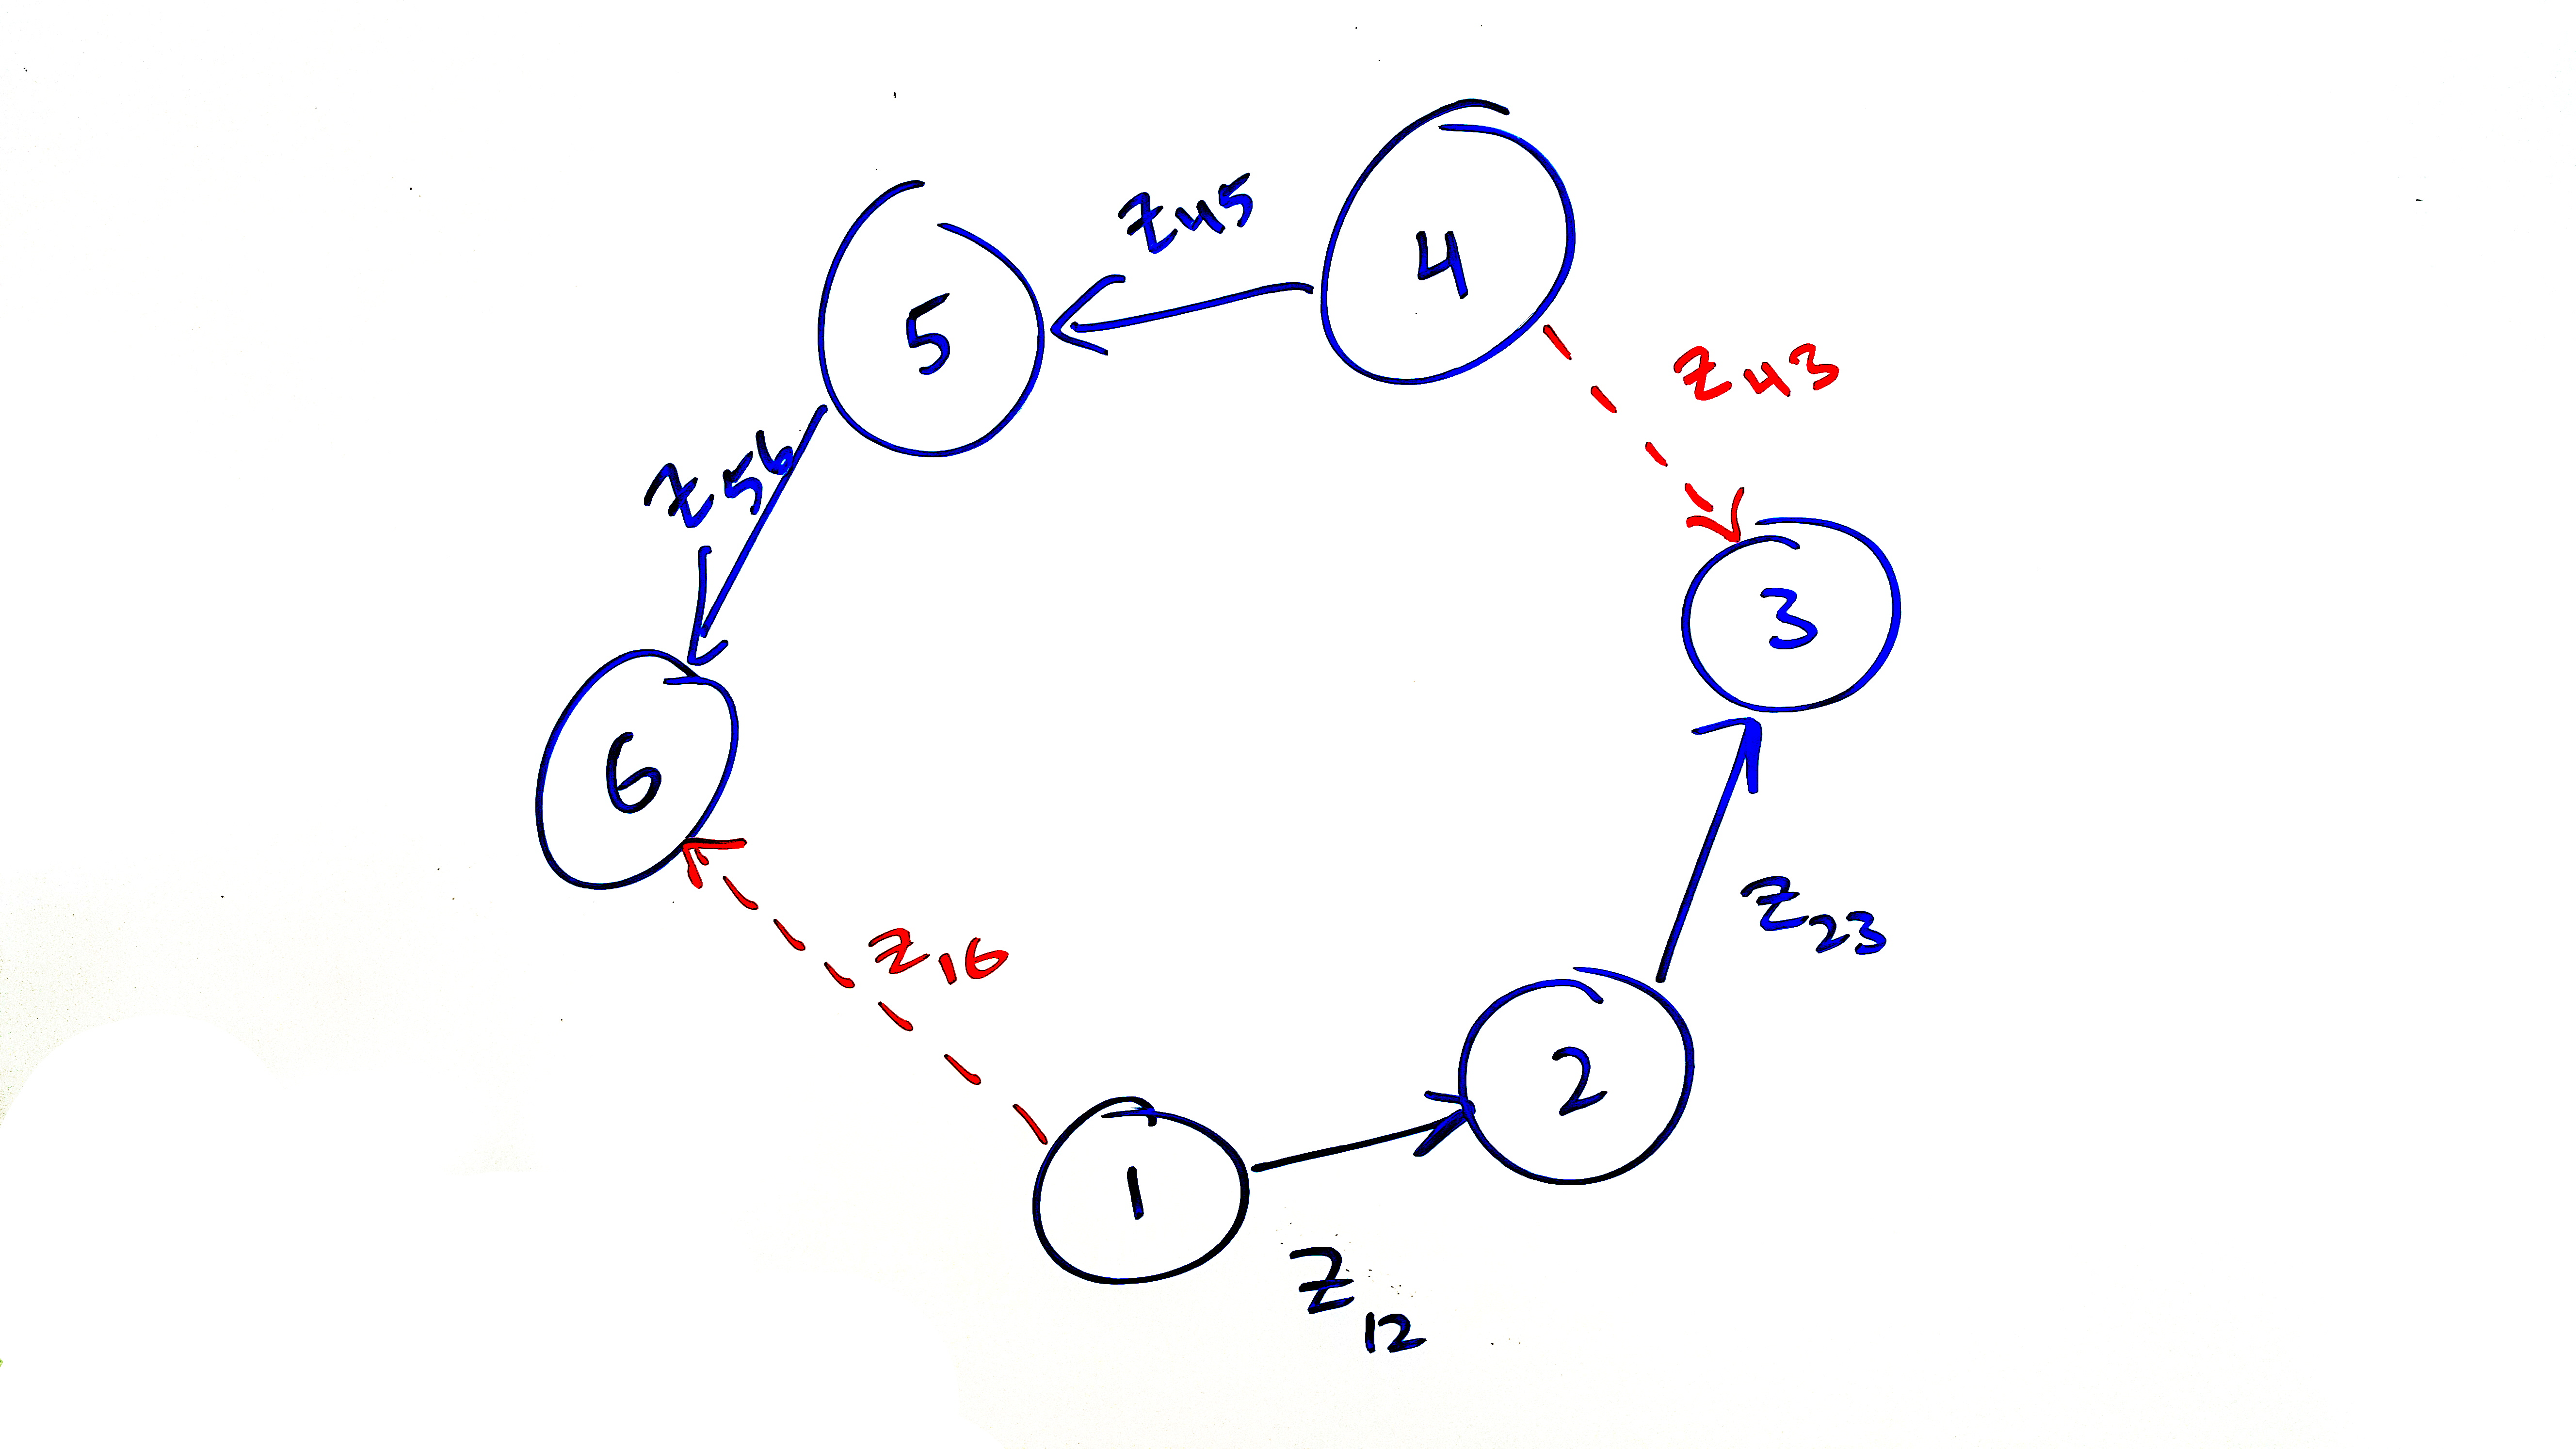
\includegraphics[width=0.7\textwidth]{figures/multiple_lc}}
\end{figure}


The compounding of edges can be described as

\[
\begin{aligned}\hat{\mathbf{z}}_{1-6} & =\hat{\mathbf{z}}_{12}\otimes\hat{\mathbf{z}}_{23}\otimes\hat{\mathbf{z}}_{43}^{-1}\otimes\hat{\mathbf{z}}_{45}\otimes\hat{\mathbf{z}}_{56}\end{aligned}
\]


First, let's just look at how the translations compound

\[
\begin{aligned}\hat{\Delta t}_{1-6} & =\hat{\Delta t}_{12}+\textrm{R}_{12}\Delta t_{23}-\textrm{R}_{12}\textrm{R}_{23}\textrm{R}_{43}^{\top}\Delta t_{43}+\textrm{R}_{12}\textrm{R}_{23}\textrm{R}_{43}^{\top}\Delta t_{45}+\textrm{R}_{12}\textrm{R}_{23}\textrm{R}_{43}^{\top}\textrm{R}_{45}\Delta t_{56}\\
\bar{\Delta t}_{16} & =\Delta t_{16}
\end{aligned}
\]


Next, a look at how rotation matrices compound (note that the heading
angle simply sums)

\[
\begin{aligned}\textrm{R}_{1-6} & =\textrm{R}_{12}\textrm{R}_{23}\textrm{R}_{43}^{\top}\textrm{R}_{45}\textrm{R}_{56}\\
\textrm{R}_{1-6} & =\textrm{R}_{\theta_{12}+\theta_{23}-\theta_{43}+\theta_{45}+\theta_{56}}\\
\textrm{R}_{16} & =\bar{\textrm{R}}_{16}
\end{aligned}
\]


Now a quick review of the calculus of rotation matrices

\[
\begin{aligned}\textrm{R}_{\theta} & =\left[\begin{array}{cc}
\cos\theta & -\sin\theta\\
\sin\theta & \cos\theta
\end{array}\right]\\
\dfrac{d\textrm{R}_{\theta}}{d\theta} & =\left[\begin{array}{cc}
-\sin\theta & -\cos\theta\\
\cos\theta & -\sin\theta
\end{array}\right]\\
\textrm{R}_{\theta}^{\prime} & =\textrm{R}_{\tfrac{\pi}{2}+\theta}
\end{aligned}
\]


\[
\begin{aligned}\textrm{R}_{\theta_{1}}^{\prime}\textrm{R}_{\theta_{2}} & =\textrm{R}_{\tfrac{\pi}{2}+\theta_{1}}\textrm{R}_{\theta_{2}}\\
 & =\textrm{R}_{\tfrac{\pi}{2}+\theta_{1}+\theta_{2}}\\
 & =\textrm{R}_{\theta_{1}+\theta_{2}+\tfrac{\pi}{2}}\\
 & =\textrm{R}_{\theta_{1}}\textrm{R}_{\theta_{2}+\tfrac{\pi}{2}}\\
 & =\textrm{R}_{\theta_{1}}\textrm{R}_{\theta_{2}}^{\prime}
\end{aligned}
\]


\[
\begin{aligned}\textrm{R}_{\theta_{1}}^{\prime}\textrm{R}_{\theta_{2}}^{\top} & =\textrm{R}_{\tfrac{\pi}{2}+\theta_{1}}\textrm{R}_{\theta_{2}}^{\top}\\
 & =\textrm{R}_{\tfrac{\pi}{2}+\theta_{1}-\theta_{2}}\\
 & =\textrm{R}_{\theta_{1}-\theta_{2}+\tfrac{\pi}{2}}\\
 & =\textrm{R}_{\theta_{1}}\textrm{R}_{\theta_{2}-\tfrac{\pi}{2}}^{\top}\\
 & =-\textrm{R}_{\theta_{1}}\textrm{R}_{\theta_{2}}^{\prime\top}
\end{aligned}
\]


Finally, calculate the Jacobian $\frac{\partial\hat{\mathbf{z}}_{1-6}}{\partial\mathbf{z}}$

\[
\begin{aligned}\frac{\partial\hat{\Delta t}_{1-6}}{\partial\Delta t_{12}} & =1\\
\frac{\partial\hat{\Delta t}_{1-6}}{\partial\Delta t_{23}} & =\textrm{R}_{12}\\
\frac{\partial\hat{\Delta t}_{1-6}}{\partial\Delta t_{43}} & =-\textrm{R}_{12}\textrm{R}_{23}\textrm{R}_{43}^{\top}\\
\frac{\partial\hat{\Delta t}_{1-6}}{\partial\Delta t_{45}} & =\textrm{R}_{12}\textrm{R}_{23}\textrm{R}_{43}^{\top}\textrm{R}_{45}\\
\frac{\partial\hat{\Delta t}_{1-6}}{\partial\Delta t_{56}} & =\textrm{R}_{12}\textrm{R}_{23}\textrm{R}_{43}^{\top}\textrm{R}_{45}\textrm{R}_{56}\Delta t_{56}
\end{aligned}
\]


\[
\begin{aligned}\frac{\partial\hat{\Delta t}_{1-6}}{\partial\theta_{12}} & =\partial(\Delta t_{12}+\textrm{R}_{12}\Delta t_{23}-\textrm{R}_{12}\textrm{R}_{23}\textrm{R}_{43}^{\top}\Delta t_{43}+\textrm{R}_{12}\textrm{R}_{23}\textrm{R}_{43}^{\top}\Delta t_{45}+\textrm{R}_{12}\textrm{R}_{23}\textrm{R}_{43}^{\top}\textrm{R}_{45}\Delta t_{56})/\partial\theta_{12}\\
 & =\textrm{R}_{12}^{\prime}\Delta t_{23}-\textrm{R}_{12}^{\prime}\textrm{R}_{23}\textrm{R}_{43}^{\top}\Delta t_{43}+\textrm{R}_{12}^{\prime}\textrm{R}_{23}\textrm{R}_{43}^{\top}\Delta t_{45}+\textrm{R}_{12}^{\prime}\textrm{R}_{23}\textrm{R}_{43}^{\top}\textrm{R}_{45}\Delta t_{56}\\
 & =\textrm{R}_{\frac{\pi}{2}+\theta_{12}}\Delta t_{23}-\textrm{R}_{\frac{\pi}{2}+\theta_{12}+\theta_{23}-\theta_{43}}\Delta t_{43}+\textrm{R}_{\frac{\pi}{2}+\theta_{12}+\theta_{23}-\theta_{43}}\Delta t_{45}+\textrm{R}_{\frac{\pi}{2}+\theta_{12}+\theta_{23}-\theta_{43}+\theta_{45}}\Delta t_{56}\\
\frac{\partial\hat{\Delta t}_{1-6}}{\partial\theta_{23}} & =\partial(\Delta t_{12}+\textrm{R}_{12}\Delta t_{23}-\textrm{R}_{12}\textrm{R}_{23}\textrm{R}_{43}^{\top}\Delta t_{43}+\textrm{R}_{12}\textrm{R}_{23}\textrm{R}_{43}^{\top}\Delta t_{45}+\textrm{R}_{12}\textrm{R}_{23}\textrm{R}_{43}^{\top}\textrm{R}_{45}\Delta t_{56})/\partial\theta_{23}\\
 & =-\textrm{R}_{12}\textrm{R}_{23}^{\prime}\textrm{R}_{43}^{\top}\Delta t_{43}+\textrm{R}_{12}\textrm{R}_{23}^{\prime}\textrm{R}_{43}^{\top}\Delta t_{45}+\textrm{R}_{12}\textrm{R}_{23}^{\prime}\textrm{R}_{43}^{\top}\textrm{R}_{45}\Delta t_{56}\\
 & =-\textrm{R}_{\frac{\pi}{2}+\theta_{12}+\theta_{23}-\theta_{43}}\Delta t_{43}+\textrm{R}_{\frac{\pi}{2}+\theta_{12}+\theta_{23}-\theta_{43}}\Delta t_{45}+\textrm{R}_{\frac{\pi}{2}+\theta_{12}+\theta_{23}-\theta_{43}+\theta_{45}}\Delta t_{56}\\
\frac{\partial\hat{\Delta t}_{1-6}}{\partial\theta_{43}} & =\partial(\Delta t_{12}+\textrm{R}_{12}\Delta t_{23}-\textrm{R}_{12}\textrm{R}_{23}\textrm{R}_{43}^{\top}\Delta t_{43}+\textrm{R}_{12}\textrm{R}_{23}\textrm{R}_{43}^{\top}\Delta t_{45}+\textrm{R}_{12}\textrm{R}_{23}\textrm{R}_{43}^{\top}\textrm{R}_{45}\Delta t_{56})/\partial\theta_{43}\\
 & =-\textrm{R}_{12}\textrm{R}_{23}\textrm{R}_{43}^{\prime\top}\Delta t_{43}+\textrm{R}_{12}\textrm{R}_{23}\textrm{R}_{43}^{\prime\top}\Delta t_{45}+\textrm{R}_{12}\textrm{R}_{23}\textrm{R}_{43}^{\prime\top}\textrm{R}_{45}\Delta t_{56}\\
 & =-\textrm{R}_{\theta_{12}+\theta_{23}-(\frac{\pi}{2}+\theta_{43})}\Delta t_{43}+\textrm{R}_{\theta_{12}+\theta_{23}-(\frac{\pi}{2}+\theta_{43})}\Delta t_{45}+\textrm{R}_{\theta_{12}+\theta_{23}-(\frac{pi}{2}+\theta_{43})+\theta_{45}}\Delta t_{56}\\
 & =-\textrm{R}_{-\frac{\pi}{2}+\theta_{12}+\theta_{23}-\theta_{43}}\Delta t_{43}+\textrm{R}_{-\frac{\pi}{2}+\theta_{12}+\theta_{23}-\theta_{43}}\Delta t_{45}+\textrm{R}_{-\frac{\pi}{2}+\theta_{12}+\theta_{23}-\theta_{43}+\theta_{45}}\Delta t_{56}\\
\frac{\partial\hat{\Delta t}_{1-6}}{\partial\theta_{45}} & =\partial(\Delta t_{12}+\textrm{R}_{12}\Delta t_{23}-\textrm{R}_{12}\textrm{R}_{23}\textrm{R}_{43}^{\top}\Delta t_{43}+\textrm{R}_{12}\textrm{R}_{23}\textrm{R}_{43}^{\top}\Delta t_{45}+\textrm{R}_{12}\textrm{R}_{23}\textrm{R}_{43}^{\top}\textrm{R}_{45}\Delta t_{56})/\partial\theta_{45}\\
 & =\textrm{R}_{12}\textrm{R}_{23}\textrm{R}_{43}^{\top}\textrm{R}_{45}^{\prime}\textrm{R}_{56}\Delta t_{56}\\
 & =\textrm{R}_{\frac{\pi}{2}+\theta_{12}+\theta_{23}-\theta_{43}+\theta_{45}+\theta_{56}}\Delta t_{56}\\
\frac{\partial\hat{\Delta t}_{1-6}}{\partial\theta_{56}} & =\partial(\Delta t_{12}+\textrm{R}_{12}\Delta t_{23}-\textrm{R}_{12}\textrm{R}_{23}\textrm{R}_{43}^{\top}\Delta t_{43}+\textrm{R}_{12}\textrm{R}_{23}\textrm{R}_{43}^{\top}\Delta t_{45}+\textrm{R}_{12}\textrm{R}_{23}\textrm{R}_{43}^{\top}\textrm{R}_{45}\Delta t_{56})/\partial\theta_{56}\\
 & =0
\end{aligned}
\]


\[
\begin{aligned}\frac{\partial\theta_{1-6}}{\partial\theta_{12}} & =\partial(\theta_{12}+\theta_{23}-\theta_{43}+\theta_{45}+\theta_{56})/\partial\theta_{12}\\
 & =1\\
\frac{\partial\theta_{1-6}}{\partial\theta_{23}} & =1\\
\frac{\partial\theta_{1-6}}{\partial\theta_{43}} & =-1\\
\frac{\partial\theta_{1-6}}{\partial\theta_{45}} & =1\\
\frac{\partial\theta_{1-6}}{\partial\theta_{56}} & =1
\end{aligned}
\]

\end{document}
